\cmpd*{da, amda, mon, moni, schifo, dmon, dhn, clorofosfito, legante, pba, nc, ncb} %ho dovuto metterlo sennò chemnum li ordinava in base alla prima figura in cui compariva \cmpdref e non alla prima volta che compariva \cmpd. Molto fastidioso. Servirebbe una opzione che dice: i \cmpdref non dichiarano il composto, oppure servirebbe l'esistenza di \cmpdref+ e \cmpdref+-





\chapter{Introduction}
%\sub
%\section{The Asymmetric Synthesis}
In this laboratory report is illustrated the work done by Ilario Gelmetti and Andrea Leoncini in the period of november 2011 in Prof. Anna Iuliano's laboratory in the Department of Chemistry and Industrial Chemistry of the University of Pisa. Our work was aimed to the synthesis and use of a chiral phosphite ligand for rhodium (I) as active asymmetric catalyst.

The cheapness in obtaining chiral products is of pivotal importance in the synthesis of the vast majority of drugs.
\paragraph{The Asymmetric Synthesis}
In order to obtain an enantiomerically enriched product starting from a prochiral one is necessary to introduce an external source of chirality: chiral solvent, chiral auxiliary\footnote{Chiral auxiliary: a chiral reagent that is temporarily incorporated in order to switch the reaction from enantioselective to diastereoselective and then removed from the product, a stoichiometric amount is needed.} 
 or chiral catalyst. We will use a chiral catalyst, which is the most frequently used way and cheaper than other strategies due to the smaller amount of chiral compound required. In particular, this is true when the catalyst can be prepared without chiral resolution or prepared from chiral moieties naturally available in the pure form.
\paragraph{Chiral catalyst} Usually the core of a catalyst is a metallic atom, so the chirality during the reactions has to be induced by the presence of the chiral ligands. This ligands have to remain coordinated to the metal center during the transformation of the substrates to the products and have to exert an influence (often a steric effect or other interactions) on the reacting species, usually on the transition states, so that we have two diastereomeric forms with different energies and the product deriving from the most stable will be the main product.
\paragraph{Ligands} Chirality is often introduced by chiral cavities or rigid biarylic systems (rigidity and $C_{2}$ symmetry decrease the degrees of freedom and so the number of possible transition states and products). A rigid - \emph{atropos} - biarylic ligand is usually expensive to obtain in a enantiopure formulation (mainly because its synthesis would require chiral reagents and/or chiral resolution). A cheaper and easier way employs a flexible - \emph{tropos} -  biarylic system in which a preferential rotation is induced by a chiral molecule abundant in nature.

%to induce a sufficient difference in energy between the formed diastereoisomeric forms are used
  

%In generale si possono ottenere reazioni stereoselettive solamente lavarando in un ambinte chirale. Questo può essere ottenuto con reagenti chirali o con catalizzatori asimmetrici.

%Il principale problema legato all'impiego di reagenti chirali è che questi devono essere utilizzati in quantità stechiometrica. Dal punto di vista sintetico ed economico, l'uso di catalizzatori asimmetrici è vantaggioso perchè è possibile ottenere reazioni asimmetriche con reagenti achirali, meno costosi dei reagenti chirali.

%Per avere sintesi asimmetriche è necessario passare attraverso stati di transizione chirali. Nel caso di impiego 0di complessi di metalli di transizione come sistemi catalitici, il complesso può essere reso chirale usando leganti chirali.

% In generale condizioni che aiutano l'induzione asimmetrica sono sistemi biarilici, cavità chirali e leganti "rigidi". La rigidità del legante e la simmetria $C_{2}$ riducono le conformazioni distinte che possono assumere i leganti, riducendo il numero di stati di transizione diversi.
% Con reagenti chirali il problema è che vanno usati in quantità stechiometrica. Questi sistemi non sono più usati, perché al loro posto è più conveniente usare dei catalizzatori asimmetrici.
% Per avere sintesi asimmetriche è necessario avere dei complessi chirali, che possono essere resi tali con dei leganti chirali.
% Condizioni che aiutano l'induzione asimmetrica sono sistemi biarilici, cavità chirali e leganti “rigidi” (conformazionalmente omogenei; riducendo le conformazioni dei leganti si riducono gli stati di transizione)


%\sub
%\section{Tropos  and Deoxycholic Acid}
\paragraph{Ligands: \emph{Tropos versus Atropos}}
For our study on the reaction exposed in Figure \ref{sc:tutto-riassunto} we'll use a trisubstituited phosphite as chiral ligand for the rhodium metallic center. In this system chirality has to lie only on phosphite substituents. Following the success of bi\-naphthylic atrop\-isomeric systems in chiral catalysis (like 1,1'-bi\-naphthyl 2,2'-bis substituted systems) we decided to prepare a novel ligand, the 2,2'-bi\-naphthyl 1,1'-bis substituted.
The main disadvantage of using \emph{tropos} ligands, Figure \ref{sc:tropos}, is that they can rotate freely on their atrop\-isomeric axis, in this case the C$_1$-C$_1$', so the chirality can't be retained, Figure \ref{sc:atropos}. This turns into an advantage when a preferential atrop\-isomeric conformation can be induced by an external source of chirality. This way the problem of obtaining stereo\-chemically pure bi\-naphthyls is avoided and moved to the other source of chirality, that could occur enantiopure in nature.

The induction of chirality could be not %(può non essere quantitativa, cioè non è obbligatorio) - Leo. Ok, ma ho girato be e not - Ilario.
 quantitative (we can have a matched or a mismatched diastereoisomer); %(we have only one configuration of deoxy\-cholic group but we have both conformations of the binaphthyl group, the major diastereoisomer is called \emph{matched} and the minor \emph{mismatched})
nevertheless good enantiomeric excesses of the product can be obtained due to the different catalytic activity of the two diastereoisomeric forms of the ligand.

\ifpdf
\begin{SCfigure}
 \centering
  \subfigure[Our \emph{tropos} aromatic system.\label{sc:tropos}]{\includegraphics[width=.53\textwidth]{sc/tropos.png}}\qquad%\qquad
  \subfigure[Atropos.\label{sc:atropos}]{\includegraphics[width=.39\textwidth]{sc/atropos.png}}
\caption{\\Two molecules: \emph{tropos} and \emph{atropos}.}
\end{SCfigure}
\else
\fignoeps
\fi

\paragraph{Vaulted Ligands}
Our novel bi\-naphthyl, Figure \ref{sc:tropos}, has also another advantage over the more traditional one based on BINAP \footnote{BINAP: 2,2'-bis(diphenylphosphino)-1,1'-bi\-naphthyl}, Figure \ref{sc:atropos}: is vaulted. This fact can have beneficial effects on enantioselectivity because the chiral inducing groups come closer to the active site, the rhodium atom. This positive effect was observed by \citet{Bao1993} using \emph{atropos} ligands.
It will be possible to study the distortion in the bi\-naphthylic system comparing results from circular dichroism and theoretical computations.


% É stato osservato che l'impiego di unità chirali di genere diverso (assiale e configurazionale) favorisce eccessi enantiomerici. eeeeh? fonte?
% La natura flessibile delle unità \emph{tropos} risulta in uno spostamento dell'equilibrio fra le due forme diastereomeriche verso quella più stabile, 
%%% determinando così la prevalenza di una specie in soluzione e quindi il raggiungimento di elevati livelli di induzione asimmetrica.
% 
% Il tipo di leganti che andremo a preparare sono atrop\-isomerici. Sono a tutti gli effetti chirali anche se non hanno carboni asimmetrici. Composti che si possono trovare in conformazioni chirali, come il bifenolo, prendono il nome di composti di tipo \emph{tropos}.


% 2,2' perché più facile che siano \emph{tropos}. 1,1' hanno già gli H in 8,8' a rompere le balle
% perché non è mai stato fatto il 2,2'
% 
% Se l'alcol usato (chirale) non passa attraverso la risoluzione enantiomerica otteniamo dei leganti chirali senza passare mai attraverso una risoluzione [il fosfito biarilico non viene risolto]  rimosse le lunghe e dispendiose procedure di risoluzione di composti biarilici racemi.



\paragraph{Deoxycholic acid}
The natural, cheap, chiral compound we chose as source of chirality is 7-deoxy\-cholic acid \cmpd+{da} which is a byproduct of intestinal bacterial digestion 
derived from cholic acid, one of the bile acids secreted by the liver. It presents two alcoholic functional groups (on C-12 and C-3) and a carboxylic acid group (on C-24). 
As we can see in Figure \ref{fig:deoxycholic3d} the configuration of this molecule is folded so that the alcoholic group in position 12 is in a cavity. \label{dodici}
The conformation of an \emph{atropos} substituent in that position would be affected by the steric effects of the cavity.

\begin{SCfigure}
 \centering
  \cmpdref-{da}
  \subfigure[The structure.\label{fig:deoxycholic}]{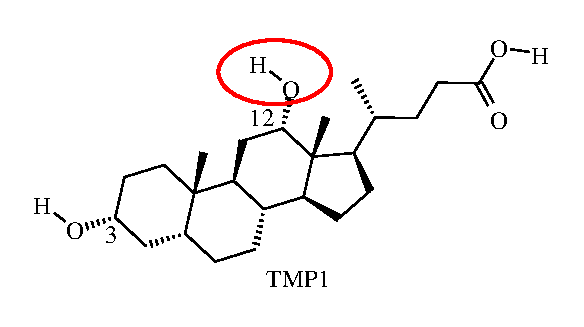
\includegraphics[width=.4\textwidth]{mol/deoxycholic.eps}}%\qquad\qquad
  \ifpdf
  \subfigure[\footnotesize{3D view of 7-deoxy\-cholic acid with emphasis on alcoholic group in position 12. Optimized using Gaussian 09c01 semi-empirical PM6.}\label{fig:deoxycholic3d}]{\includegraphics[width=.55\textwidth]{mol/deoxycholic3d-small.png}}
  \else
  \noeps
  \fi
\caption{\\The 7-deoxy\-cholic acid.}
\end{SCfigure}

% \begin{figure}			%schema nel quale lavora il pacchetto per mettere i numeri
% \centering{
% \cmpdref-{deoxy\-cholic}
% \includegraphics{mol/deoxy\-cholic.eps}
% \caption{Deoxycholic acid.\label{sc:deoxy\-cholic}}
% }
%  \end{figure}

% 				%questo sotto è il modo per evitare problemi facendo latex/pdflatex
% \ifpdf				%il pacchetto controlla se esegue pdflatex o latex
% \begin{figure}		%se va pdflatex mette l'immagine normalmente
%  \centering
%  \includegraphics[width=.7\textwidth]{mol/deoxy\-cholic3d-small.png}
%   \caption{3D view of deoxy\-cholic acid.\label{fig:deoxy\-cholic3d}}
% \end{figure}
% \else				%se va latex mette il segnaposto per l'immagine
% \fignoeps
% \fi




% 
% Saranno usati derivati degli acidi biliari. La struttura tridimensionale è rigida  e concava.
% [riferito alla struttura dello scheletro steroideo]
% i gruppi OH sono tutti rivolti verso la parte concava. Una funzionalizzazione di questi ossidrili crea una cavità altamente asimmetrica.
% Inoltre i tre ossidrili sono molto diversi e possono essere derivatizzati selettivamente. I migliori derivati sono quelli con la funzionalizzazione in 12. Si usa quindi l'acido deossicolico (che è quello senza l'OH in 7)

% lo scheletro steroideo degli acidi colico e deossicolico è capace di indurre un senso prevalente di torsione all'unità bifenilfosfitica, dipendente dalla posizione in cui questa è legata allo scheletro steroideo, e leganti chirali efficienti per le reazioni asimmetriche sono stati ottenuti legando le unità bifenilfosfitiche alla posizione 12 dell'acido deossicolico.
% 
% Per vedere se l'acido ha indotto una prevalenza di conformazione del fosfito si può usare il dicroismo circolare.
% 
% Una volta ottenuti gli spettri CD, per ricavare quale conformazione ha il sistema biarilico si usa un calcolo QM dello spettro CD.
% 
% [dopo il discorso sugli spettri CD]
% Il sistema biarilico quindi è in equilibrio (cambia torsione in base al solvente). Fornisce ottimi eccessi enantiomerici nonostante una bassa induzione i conformazione (circa 60:40). DA DOVE VIENE LA PROPORZIONE? DALL'NMR? CE L'ABBIAMO?
% 
% 
% Facendo lo spettro P-NMR a temperatura variabile del complesso si osserva che si ottiene una miscela 50:50 delle due conformazioni. Però una delle due non è attiva nella catalisi.
% Durante la reazione l'equilibrio si sposta verso la forma attiva perché una parte entra nel ciclo catalitico. Questo è possibile solo perché è un sistema \emph{tropos}. BAH...






%\sub
%\section
\paragraph{Addition of %Aryl
Boronic Acids to Enones}
%L'addizione coniugata di acidi boronici a enoni catalizzata da complessi di rodio (I)}
In 1997 \citet{Sakai1997} discovered the reaction of conjugate addition of substituted arylboronic acid to acyclic enones, as summarized in 
Figure \ref{sc:1997-generico}, in aqueous environment using a combination of \ce{(acac)Rh(CO)2} and \ce{dppb}.

\ifpdf
\begin{SCfigure}%[h]
 \centering
 \includegraphics[width=.8\textwidth]{sc/1997-generico.png}
  \caption{\\The original reaction by \citet{Sakai1997}. \label{sc:1997-generico}}
\end{SCfigure}
\else
\fignoeps
\fi


\paragraph{Organoboronic Acids} Organoboronic acids are convenient organometallic reagents: they are stable to moisture and to oxygen. They are not so reactive toward enones in the absence of a rhodium catalyst and no 1,2-addition to enones takes place neither with nor without the catalyst. 

%tolgo perché si dice nel prossimo capitolo che non è detto che la base sia importante per quello.
%When the reaction is performed in basic aqueous environment, as suggested in Figure \ref{sc:1998-OH}, the boronic acid is in its quaternized form and therefore is more reactive.

\paragraph{The Asymmetric Version} In 1992 \citet{Rossiter1992} reviewed some early methods of conjugate addition of organometal reagents to enones using chiral catalysts.  %1993 \citet{Alexakis1993} discovered an asymmetric addition of organocopper reagents to a cyclic enone involving a chiral phosphorous ligand. 
\citet{Miyaura1998} discovered the asymmetric version of the addition of boronic acids to enones using \emph{atropos} BINAP %\footnote{BINAP: 2,2'-bis(diphenylphosphino)-1,1'-bi\-naphthyl} la nota l'ho messa alla prima ricorrenza di ``BINAP'' - Leo
as a bidentate ligand: the proposed mechanism is shown in Figure \ref{sc:1998-OH}. As shown in the figure the key step for stereoselectivity is the direction of approach of the enone towards the catalyst, which is regulated by the ligands. Nowadays monodentate ligands are more common due to their cheaper and easier synthesis, compared to bidentate ligands. 
%In this laboratory is known that for the reaction of interest the more appropriate ratio between monodentate ligand and rhodium(I) atom is 1 to 1; in the same reaction the group of \citet{Gennari2007} tested the ratio 2 to 1 in which they used pair of different monodentated chiral \emph{tropos} phosphite ligands.
In this laboratory is known that a 2 to 1 ratio between monodentate ligand and rhodium(I) atom is more often successful in reaching a good yield and enantiomeric excess (2 to 1 ratio has been used also by \citet{Gennari2007} 
but with a pair of different monodentate chiral \emph{tropos} phosphite ligands).
\ifpdf
\begin{SCfigure}
 \centering
 \includegraphics[width=.6\textwidth]{sc/1998-OH.png}
  \caption{\\ The proposed mechanism for the reaction using dppb as ligand. The bi\-naphthylene moiety in (S)-binap is omitted for clarity.
\label{sc:1998-OH}}
\end{SCfigure}
\else
\fignoeps
\fi

\paragraph{Stereo\-selective Addition of Boronic Acids to Nitro Alkenes}
1-Nitro\-alkenes are interesting substrates for conjugate addition due to the variety of functional groups achievable starting from the nitro group present in the product. Moreover, 1-nitro\-alkenes behave almost like $\alpha$,$\beta$-un\-saturated carbonyls, but cannot react in positions 1-2. There have been very few reports on the asymmetric addition of boronic acids to 1-nitro\-alkenes $\alpha$-substituted \cite{Hayashi2000} and $\alpha$-unsubstituted \cite{Wang2010, Xue2012}. In each case a rhodium catalyst was used in addition to a variety of chiral ligands. The presence of a substituent in $\alpha$ position of the double bond in 1-nitro-cyclo\-hexene allows to study the relative stereo\-chemistry at $\alpha$ and $\beta$ positions. A prevalence for the thermo\-dynamically less stable \emph{cis} product and a good diastereo\-selectivity was reported \cite{Hayashi2000}. 

\paragraph{Our Work} The goal of this work is to perform an asymmetric addition of phenylboronic acid to a cyclic electron-poor olefin. We have synthesized a novel monodentate ligand, the phosphite \cmpd+{legante} in 
Figure \ref{fig:legante}, using 1-methoxy\-naphthalene \cmpd+{mon}%numeriamo anche questi qua inutili materiali di partenza?
, 7-deoxy\-cholic acid \cmpd+{da}, \ce{PCl3} and methyl acetate as starting materials. Then we have used this novel ligand in a ligand exchange on rhodium 
that was subsequently used in the reaction of asymmetric addition of phenylboronic acid \cmpd+{fba} to 1-nitro\-cyclo\-hexene \cmpd+{nc}. The whole work is schematized in Figure \ref{sc:tutto-riassunto}. %The synthetic steps are illustrated in Figure \ref{sc:globale}.



\begin{SCfigure}

\cmpdref-{legante}
\centering{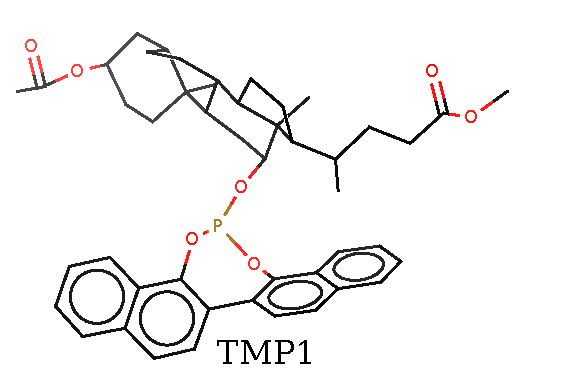
\includegraphics[width=.6\textwidth]{mol/legante.eps}}
\caption{\\ Our \emph{tropos} ligand \cmpd+{legante}. The upper part is the protected deoxy\-cholic acid \cmpd+{amda}.\label{fig:legante}}

\end{SCfigure}

\begin{SCfigure}
\centering{
 \cmpdref-{mon}
 \cmpdref-{moni}
 \cmpdref-{dmon}
 \cmpdref-{dhn}
 \cmpdref-{da}
 \cmpdref-{amda}
 \cmpdref-{legante} 
 \cmpdref-{pba}
 \cmpdref-{nc}
 \cmpdref-{ncb}
 \cmpdref-{schifo}
 \cmpdref-{clorofosfito}
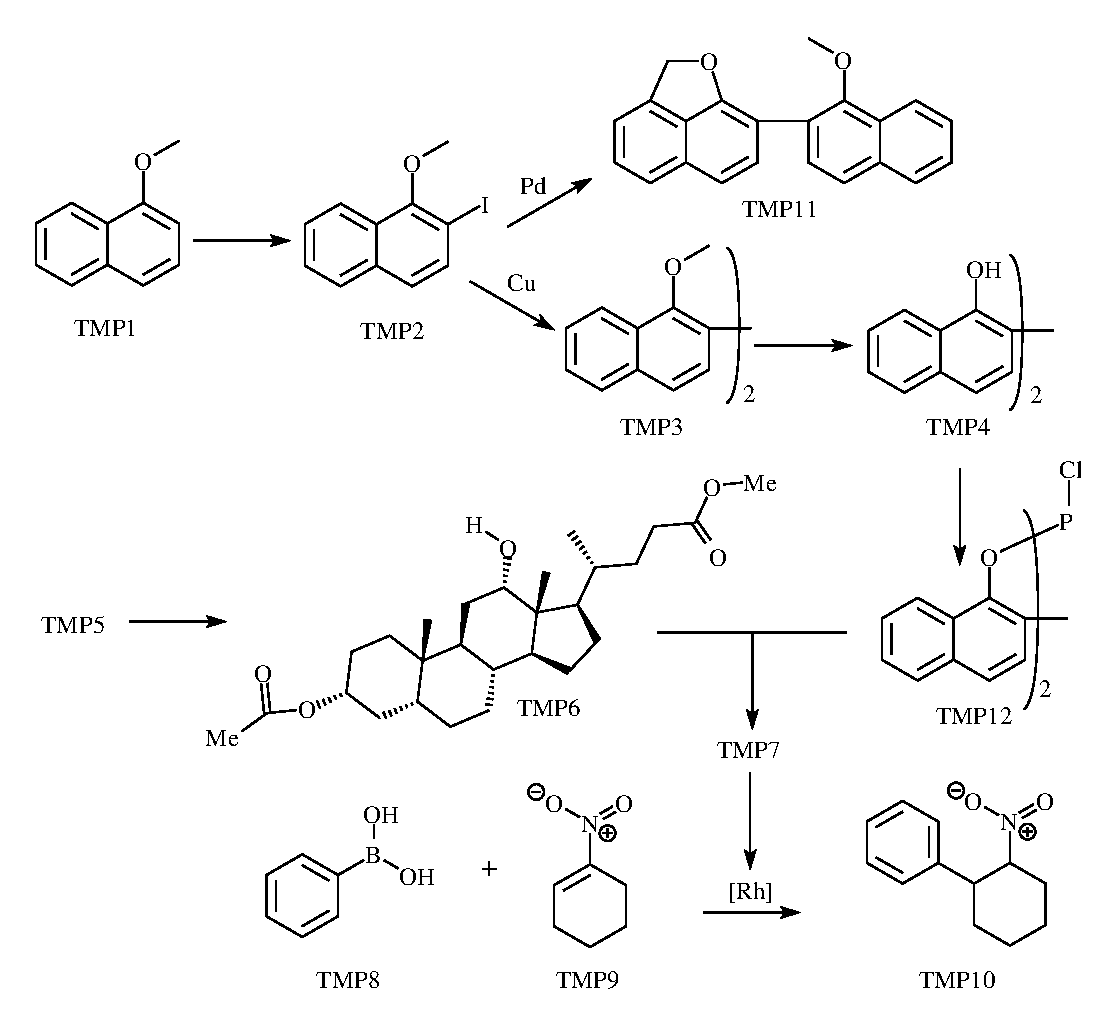
\includegraphics[width=1\textwidth]{sc/tutto-CuPd-riassunto.eps}
\caption{\\Scheme of the whole work.\label{sc:tutto-riassunto}}
}
\end{SCfigure}



% \begin{figure}
% \centering{
% \cmpdref-{fba}
% \cmpdref-{nc}
% \cmpdref-{ncb}
% \includegraphics{sc/addizione.eps}
% \caption{The target reaction.\label{sc:addizione}}
% }
%  \end{figure}
% 
% La reazione che sarà presa in considerazione in laboratorio sarà l'addizione coniugata di acidi arilboronici a doppi legami elettronpoveri (enoni).
% [schema reazione]
% Gli acidi arilboronici sono comodi: stabili in acqua e all'aria, facili da preparare, commerciali, facilmente conservabili.
% [schema reazione]
% Inoltre il B trasmetalla bene con Rh. FONTE?
% L'acido arilboronico deve essere usato in quantità sovrastechiometriche perché si può avere la reazione parassita di protodeboronazione (ArB(OH)2 → Ar-H.
%MECCANISMO


% [in riferimento al passaggio del ciclo catalitico di addizione asimmetrica coniugata]
% questo è il passaggio fondamentale. In base alla faccia con cui si lega l'enone cambia il risultato finale. Il compito di regolare la faccia con cui si lega l'enone è dei leganti.
% I leganti monodentati sono diventati molto comuni a partire dal 2003/04.
% I fosfiti monodentati semplificano molto la vita in fase di sintesi e manipolazione.
% facilità di preparazione del legante monodentato rispetto a quello bidentato
% Il complesso monosostituito è termodinamicamente più stabile, mentre quello disostituito lo è cineticamente. Si possono formare solamente scegliendo il rapporto metallo-legante. 

%Indagini spettroscopiche effettuate su miscele fra 1 e [{RhCl(C2H4)2}2] a rapporti molari 1/Rh di 1:1 e 2:1 hanno mostrato inequivocabilmente che possono essere ottenuti due differenti complessi, agenti in maniera diversa come catalizzarori della reazione.
%Il complesso monosostituito catalizza l'addizione coniugata di acidi fenilboronici a cicloesenone in modo enentioselettivo, mentre in presenza del complesso disostituito l'addizione coniugata o una doppia addizione asimmetrica, che porta a 1,3-difenilcicloesanolo, avvengono in modo dipendente dalle condizioni di reazione.

%Lo stadio determinante ai fini dell’enantioselettività è la coordinazione del doppio legame al centro metallico, momento in cui si determina quale delle due facce enantiotopiche subirà l’attacco dell’arilrodio.


% \begin{figure}\centering{ %sistema vecchio per mettere i numeri delle molecole sulle immagini
% \begin{picture}(300,200)%
%     \put(0,0){\includegraphics[width=200pt]{fosfito-finale-YEAH.pdf}}%
%     \put(90,15){\cmpd{finale}}%
% \end{picture}}
% \end{figure}

